\documentclass{beamer}
\usetheme{default}
\usepackage{verbatim}
\setbeamertemplate{navigation symbols}{}

\title{NoSQL Databases}

\author{Joshua Eckroth}

\institute{\url{http://www.cse.ohio-state.edu/~eckroth/nosql-guide.pdf}}

\date{}

\begin{document}

\begin{frame}[plain]
  \titlepage
\end{frame}

\begin{frame}{Outline}
  \tableofcontents
\end{frame}

\section{CAP theorem, ACID, BASE}

\begin{frame}{CAP theorem}

  From Eric Brewer, 2000.

  \begin{itemize}
  \item \textbf{Consistency}: all nodes see the same data at the same
    time
  \item \textbf{Availability}: every query returns a response
  \item \textbf{Partition tolerance}: continues to operate if nodes
    fail or message loss, or nodes are added/removed
  \item \textbf{Pick 2.}
  \end{itemize}

  E.g., if you want to scale up (A+P), must give up on consistency~(C).

\end{frame}

\begin{frame}{ACID}

  Regarding a transaction,

  \begin{itemize}
  \item \textbf{Atomicity}: all or nothing
  \item \textbf{Consistency}: transaction does not violate foreign key
    checks or other constraints
  \item \textbf{Isolation}: executing many transactions concurrently
    is same as serially; they don't interact
  \item \textbf{Durability}: completed transaction remains after power
    loss, etc. (i.e., written to disk)
  \end{itemize}

\end{frame}

\begin{frame}{ACID}

  \begin{itemize}
  \item hard to achieve if transaction spans nodes
  \item hard to achieve without locking (which is detrimental to performance)
  \item give up C+I for availability, graceful degradation, and performance
  \item maybe even give up D for extra performance
  \end{itemize}

  RDBMS's are typically ACID-compliant; NoSQL systems typically aren't.

\end{frame}

\begin{frame}{BASE}

  \begin{itemize}
  \item \textbf{Basically Available}: usually works
  \item \textbf{Soft state}: not always consistent
  \item \textbf{Eventually consistent}: reads across all nodes will
    eventually agree (if no updates happen in the meantime)
  \end{itemize}

  \vskip 0.5in

  \dots as opposed to ACID. (Obviously a ``backronym.'')

\end{frame}

\section{Key-value database}

\begin{frame}{Key-value database}

  \begin{center}
    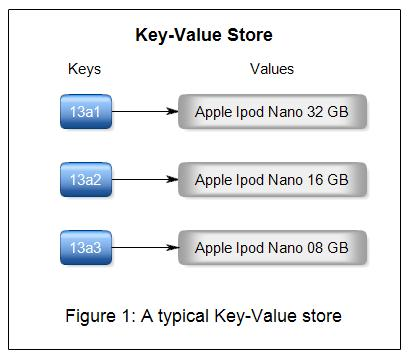
\includegraphics[width=0.5\linewidth]{key-value.jpg}
  \end{center}

  \begin{itemize}
  \item can only retrieve by a unique key
  \item just get back a value; your client code interprets the value
    (db sees it as a blob)
  \item performance is uniform and fast
  \item horizontal scaling (seems to me) straightforward
  \end{itemize}

  {\footnotesize \url{nosql.rishabhagrawal.com/2012/07/types-of-nosql-databases.html}}


\end{frame}

\begin{frame}{Key-value database}

  \textbf{Project Voldemort}

  \vskip 0.25in

  Auto-replication, auto-partitioning, ``tunable'' consistency,
  transparent failure handling.

  \vskip 0.25in

  API:

  \begin{itemize}
  \item \texttt{get(key)} --- returns a value
  \item \texttt{put(key, value)}
  \item \texttt{delete(key)}
  \end{itemize}

  \vskip 0.15in

  \url{http://www.project-voldemort.com}

\end{frame}

\begin{frame}{Key-value database}

  \textbf{Redis}

  \vskip 0.05in

  \begin{itemize}
  \item master-slave replication; a slave can become a master if the master dies
  \item supports sets, lists, dictionaries
  \end{itemize}
  
  \url{http://redis.io/}

  \vskip 0.25in

  \textbf{Memcached}

  \vskip 0.05in

  \begin{itemize}
  \item in-memory cache, never saved to disk
  \item when full, purges by LRU
  \item Facebook apparently has terabytes of ``in-memory cache''
  \end{itemize}

  \url{http://memcached.org/}

\end{frame}

\section{Document database}

\begin{frame}{Document database}

  Storage of arbitrary dictionaries that represent documents.

  \begin{itemize}
  \item also retrieved by key, or simple queries on fields
  \item data structures are stored (dictionaries \& lists, each can be nested in the other)
  \item can store a list of keys, and retrieve those recursively, in one request
  \item good for syncing (copy newer revisions; propagate deletes)
  \end{itemize}

\end{frame}

\begin{frame}[fragile]{Document database}

  Example ``document'':

\begin{verbatim}
{
 '_id':      '29a8f708e',
 '_rev':     12,
 'author':   'Josh',
 'title':    'My first blog post',
 'tags':     ['foo', 'bar'],
 'content':  'Welcome to my blog! ...',
 'backlinks': ['37dd04387', '883bc2ccd']
}
\end{verbatim}

\end{frame}

\begin{frame}{Document database}

  \textbf{MongoDB}

  \vskip 0.15in

  \begin{itemize}
  \item most popular NoSQL db
  \item easy sharding
    \begin{itemize}
    \item sharding: data subsets stored in separate machines; not
      replicated; no joins; painful in RDBMS
    \end{itemize}
  \item has some query support (find based on field values, plus some
    operators like $<$ $>$ etc.)
  \item can add indexes for faster queries
  \end{itemize}

  \vskip 0.15in
  
  \url{http://www.mongodb.org/}

\end{frame}

\begin{frame}{Document database}

  \textbf{CouchDB}

  \vskip 0.15in

  \begin{itemize}
  \item create ``views'' of the data; these are updated when docs are updated
  \item if one doc is changed by two clients, two revisions are saved;
    merging is left to the client
  \item good for offline usage; changes are sync'ed later (again, no
    default merging)
  \end{itemize}

  \vskip 0.15in

  \url{http://couchdb.apache.org/}


\end{frame}

\section{Column-family store}

\begin{frame}{Column-family store}

  \begin{center}
    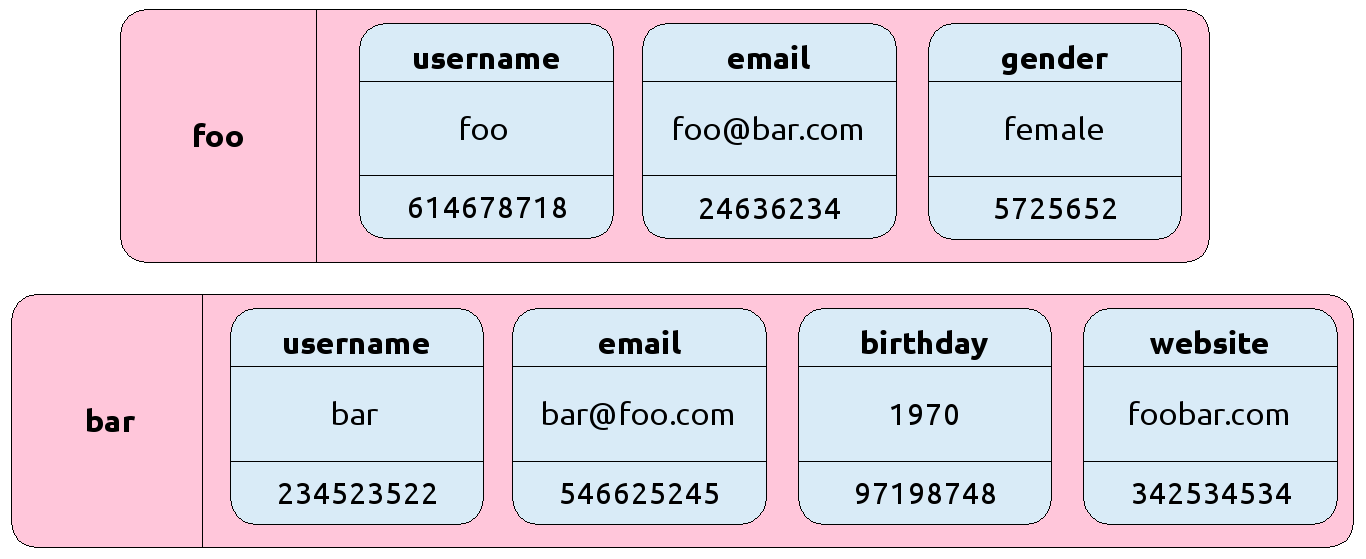
\includegraphics[width=0.8\linewidth]{excf.png}
  \end{center}

  \begin{itemize}
  \item key identifies a row in a table, which is part of 1+ column families
  \item each column family can have multiple columns
  \item values are timestamped (multiple versions of a value can be kept)
  \end{itemize}

  {\footnotesize \url{http://wikis.gm.fh-koeln.de/wiki_db/Datenbanken/Cassandra}}

\end{frame}

\begin{frame}{Column-family store}

  \textbf{Cassandra}

  \vskip 0.25in

  Very high performance. Tunable consistency. Decentralized (no
  masters). No joins or subqueries.

  \vskip 0.25in

  API:

  \begin{itemize}
  \item \texttt{get(table, key, columnName)}
  \item \texttt{insert(table, key, rowMutation)}
  \item \texttt{delete(table, key, columnName)}
  \end{itemize}

  \vskip 0.15in

  \url{http://cassandra.apache.org}

\end{frame}

\section{Graph database}

\begin{frame}{Graph database}

  Nodes + edges that connect nodes.

  \begin{itemize}
  \item each node has arbitrary relations with others
  \item each node / edge has arbitrary properties
  \item can ``walk'' or query the graph according to these relations
  \end{itemize}

  Implementations:

  \begin{itemize}
  \item \textbf{Neo4J}: \url{http://www.neo4j.org}
  \item \textbf{HyperGraphDB}: \url{http://www.hypergraphdb.org}
  \end{itemize}

\end{frame}

\begin{frame}{Graph database}

  \begin{center}
    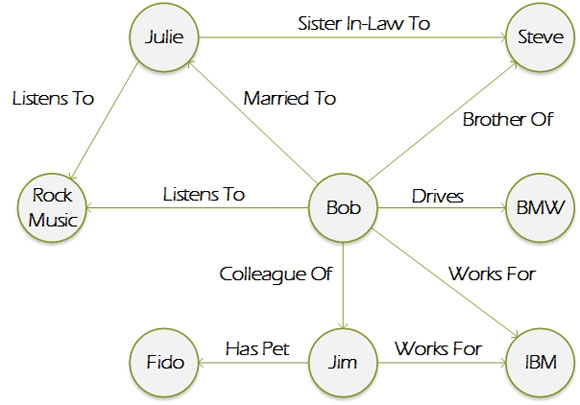
\includegraphics[width=0.8\linewidth]{Graph-database-sketch-580px.jpg}
  \end{center}
  {\footnotesize \url{http://www.computerweekly.com/feature/Whiteboard-it-the-power-of-graph-databases}}

\end{frame}

\section{Object database}

\begin{frame}[fragile]{Object database}

\begin{verbatim}
Foo f = new Foo();
db.persist(f);
for (Foo g : db.query("SELECT g FROM Foo")) {
  // do something with g...
}
\end{verbatim}

  \begin{itemize}
  \item essentially, persisting live objects
  \item basic query support, e.g., find objects of this class, etc.
  \item sometimes suffers from poor indexing, poor search, memory/disk
    fragmentation
  \end{itemize}

  Implementations:
  \begin{itemize}
  \item \textbf{db4o}: \url{http://www.db4o.com}
  \item \textbf{Cach\'{e}}: \url{http://www.intersystems.com/cache}
  \end{itemize}

\end{frame}

\section{Choosing a DB}

\begin{frame}{Choosing a DB}

Do you need ACID compliance?

{\small
\begin{center}
\begin{tabular}{c|c|c|c|c|c}
RDBMS & Key-value & Document & Column-family & Graph & Object \\
\hline
+1 & -1 & -1 & -1 & +1 & +1
\end{tabular}
\end{center}
}

Do you expect your schema to change often?

{\small
\begin{center}
\begin{tabular}{c|c|c|c|c|c}
RDBMS & Key-value & Document & Column-family & Graph & Object \\
\hline
-1 & +1 & +1 & -1 & & +1 \\
\end{tabular}
\end{center}
}

Do you expect to store terabytes / petabytes of data?

{\small
\begin{center}
\begin{tabular}{c|c|c|c|c|c}
RDBMS & Key-value & Document & Column-family & Graph & Object \\
\hline
-1 &  & -1 & +1 & +1 & \\
\end{tabular}
\end{center}
}

\end{frame}

\begin{frame}{Choosing a DB}

Do you require syncing from mobile devices?

{\small
\begin{center}
\begin{tabular}{c|c|c|c|c|c}
RDBMS & Key-value & Document & Column-family & Graph & Object \\
\hline
-1 &  & +1 & -1 & -1 & -1 \\
\end{tabular}
\end{center}
}

Do you require horizontal scaling?

{\small
\begin{center}
\begin{tabular}{c|c|c|c|c|c}
RDBMS & Key-value & Document & Column-family & Graph & Object \\
\hline
-1 & +1 & +1 & +1 & & -1 \\
\end{tabular}
\end{center}
}

Do you require extreme performance?

{\small
\begin{center}
\begin{tabular}{c|c|c|c|c|c}
RDBMS & Key-value & Document & Column-family & Graph & Object \\
\hline
-1 & +1 &  & +1 & &  \\
\end{tabular}
\end{center}
}

\end{frame}

\begin{frame}{Choosing a DB}

Do you require queries for arbitrary relations among data?

{\small
\begin{center}
\begin{tabular}{c|c|c|c|c|c}
RDBMS & Key-value & Document & Column-family & Graph & Object \\
\hline
+1 & -1 & -1 & -1 & +1 & \\
\end{tabular}
\end{center}
}

Do you want the DB to take care of complex constraints?

{\small
\begin{center}
\begin{tabular}{c|c|c|c|c|c}
RDBMS & Key-value & Document & Column-family & Graph & Object \\
\hline
+1 & -1 & -1 & -1 & -1 & \\
\end{tabular}
\end{center}
}

Do you want to save internal object state?

{\small
\begin{center}
\begin{tabular}{c|c|c|c|c|c}
RDBMS & Key-value & Document & Column-family & Graph & Object \\
\hline
+1 &  &  &  &  & +1 \\
\end{tabular}
\end{center}
}
{\footnotesize [RDBMS with Object-relational mapping (ORM)]}

\end{frame}

\section{Trends}

\begin{frame}[fragile]{Trends}


\textbf{Search trends}\\
\url{http://www.google.com/trends/explore?q=nosql#q=nosql&geo=US&date=1\%2F2009\%2049m&cmpt=q}

\vskip 0.25in

\textbf{Job trends}\\
\url{http://www.indeed.com/jobtrends?q=sql\%2C+nosql\&l=}

\vskip 0.25in

\textbf{Job trends growth}\\
\url{http://www.indeed.com/jobtrends?q=sql\%2C+nosql\&l=\&relative=1}

\end{frame}

\section{Resources}

\begin{frame}{Resources}

\textbf{Cassandra vs MongoDB vs CouchDB vs Redis vs Riak vs HBase vs
  Couchbase vs Neo4j vs Hypertable vs ElasticSearch vs Accumulo vs
  VoltDB vs Scalaris comparison} by Kristof Kovacs \\
\url{http://kkovacs.eu/cassandra-vs-mongodb-vs-couchdb-vs-redis/}

\vskip 0.15in

\textbf{NoSQL Databases}, a free book by Christof Strauch \\
\url{http://www.christof-strauch.de/nosqldbs.pdf}

\vskip 0.15in

\textbf{The NoSQL Ecosystem}, free book chapter by Adam Marcus \\
\url{http://www.aosabook.org/en/nosql.html}

\end{frame}

\end{document}
